\documentclass[final,a4paper]{article}
%%% iconv  --from-code=UTF-8 --to-code=ISO-8859-1 x.tex > x_latim.tex
%\usepackage{lucidabr}

\usepackage[T1]{fontenc}        % Permite digitar os acentos de forma normal
\usepackage[utf8]{inputenc} %% este caso o doc esteja em utf8
%% \usepackage[brazil]{babel}

\usepackage{mathtools}
%%% FOR SLIDES DIRECTly
\usepackage[ams]{pdfslide}
\usepackage{graphicx}
%%\overlay{fundo_amarelo.jpg}



%%%%%%%%%%%%%%%%%%%%%%%%%%%%%%%%%
%%\usepackage{amsmath, amsfonts ,amssymb}
%%%\usepackage{epsfig}   %float,
\usepackage[normalem]{ulem}
\usepackage{hyperref,url}
\usepackage{comment}
\usepackage{pifont}%,bbding}%%,dingbat} %%% ver manual de simbolos
\usepackage[final]{listings}

%%

\hypersetup{pdftex, colorlinks=true, linkcolor=blue, citecolor=blue, 
filecolor=blue, urlcolor=blue, pdftitle=1, pdfauthor=r4cnr, 
pdfsubject=, pdfkeywords=}
%%% COMMENT UP TO HERE .... 

%%\begin{comment}
\ifx\pdftexversion\undefined
\usepackage[dvips]{graphicx}
\else
\usepackage[pdftex]{graphicx}
\DeclareGraphicsRule{*}{mps}{*}{}
\fi
%%%\end{comment}


%\graphicspath{{./figuresdir1/}{./figuresdir2/}{./figuresdir3/}}
\graphicspath{{../../figs_genericas/}{figuras/}}

%\restylefloat{figure,table}   %%%% obrigat#io... pelo [H]
\overlay{fundo_bege.jpg}
%%salmao.png}
\pagestyle{title}


%\color{black} 


\begin{document}
%\lstset{language=Prolog}
\lstloadlanguages{Prolog,Haskell,C++}.

%\vskip 3cm
\begin{tabular}{lr}
%\vskip 2cm & {\vskip 2cm}\\

\begin{minipage}[l]{0.5\textwidth}
\vskip 2cm  %% abaixar a figura....
%%%%%%%%%%% INCLUDING PDF FIGURES
%\includegraphics[scale = 0.5]{mobius_strip_small.pdf}
%\includegraphics[scale = 1.2]{logo2_coca_icone.jpg}

\includegraphics[height=0.8\textheight, width=0.8\textwidth]{figuras/varias_distros.png}
%%\includegraphics[scale = 0.5, bb=0.0cm 6.0cm 3cm 3cm]{mobius_strip_small.pdf}
\end{minipage}
&
\begin{minipage}[r]{0.5\textwidth}

\vskip 1cm

\begin{flushleft}
 {\textsf {\Large \underline{Para Todos os Cursos}}} \\
\vskip 1cm
{\textsf {\Huge Linux: linha de comando} }\\
\vskip 1cm
{\textsf Grupo Colméia }\\ 
{\textsf Claudio Cesar de Sá}\\ 
{\textsf \$ : linha de comando}
\end{flushleft}


\end{minipage}
\end{tabular}





\section{Direitos Autorais:}
%%\textcolor{white}{xxxx}
\begin{description}

  \item[\ding{239}]  Claudio Cesar de Sá (\textsf{claudio.sa@udesc.br})
  \item[\ding{239}]  Livre para usar e melhorar
  \item[\ding{239}]  Me retorne com as melhorias! 
    \item[\ding{239}] Atualizado em \url{https://github.com/claudiosa/CCS/} $\Rightarrow $ linux
\end{description}





\tableofcontents

\section{O que é o Linux?}
\begin{itemize}
  \item Um Sistema Operacional, como Windows
  \item Código aberto -- sem proprietários
  \item Suas versões iniciais datam dos anos 199x
  \item Nome vem do idealizador: Linus Tosvalds
  \item Muitos cursos \textit{on-line} tais como:\\
  \url{https://br.udacity.com/course/linux-command-line-basics--ud595#}
\end{itemize}


\section{Linux em qualquer máquina}

\begin{figure}[!htb]
\centering
%%\includegraphics[width=0.6\textwidth , height=0.5\textheight]{figuras/trens.png}
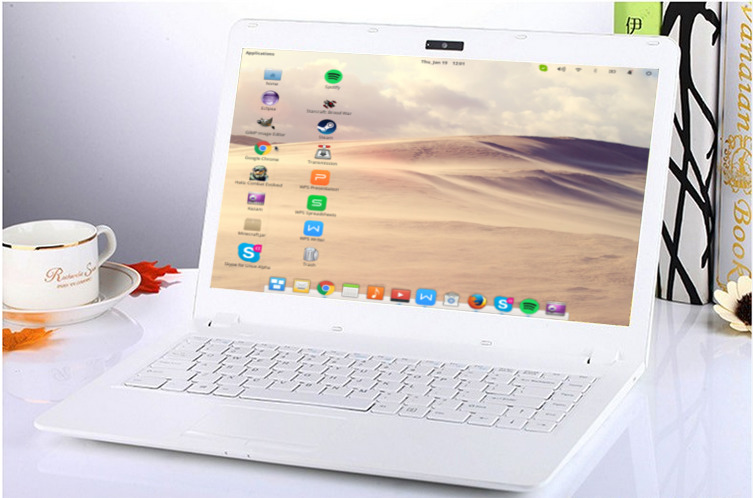
\includegraphics[width=0.6\textwidth , height=0.6\textheight]{figuras/linux-laptops-notebook.jpg}
%%%prolog/scale=0.47
%\label{fig_solutions_covering}
 \caption{Linux a U\$ 249,00}
\end{figure}





\section{Uma Interface Linux}


\begin{figure}[!htb]
\centering
%%\includegraphics[width=0.6\textwidth , height=0.5\textheight]{figuras/trens.png}
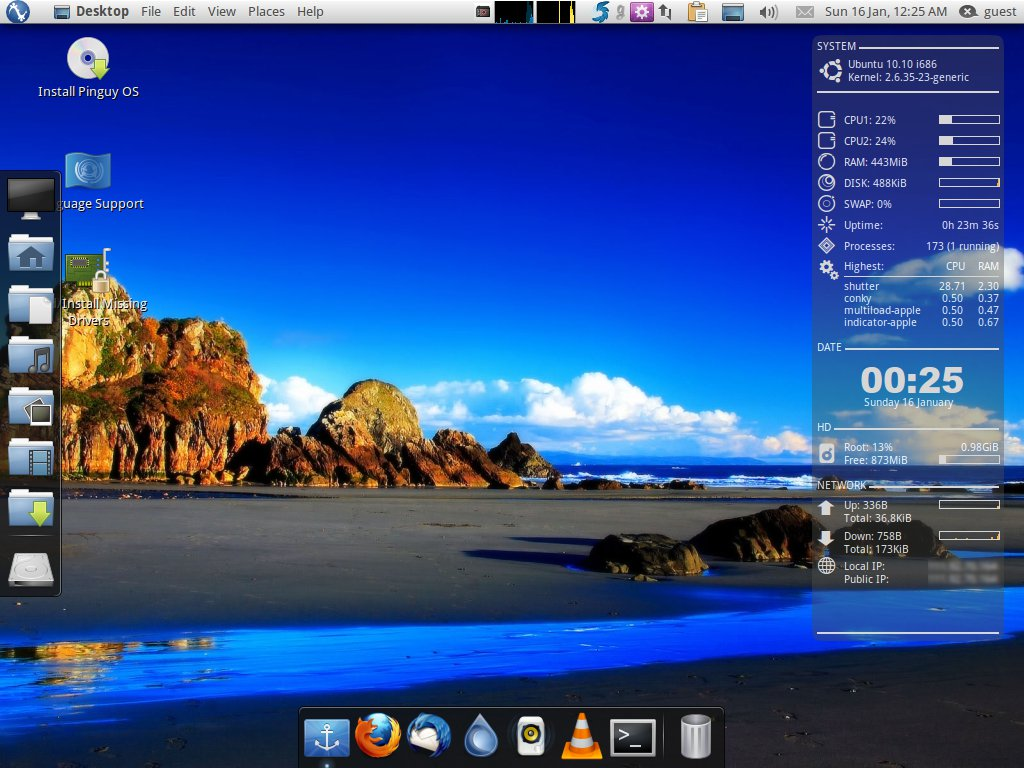
\includegraphics[scale=0.25]{figuras/desktop_linux.jpg}
%%%prolog/scale=0.47
%\label{fig_solutions_covering}
 \caption{Uma Interface Linux}
\end{figure}



\section{Linux x Hardware}

\begin{figure}[!htb]
\centering
%%\includegraphics[width=0.6\textwidth , height=0.5\textheight]{figuras/trens.png}
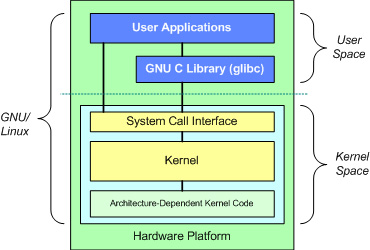
\includegraphics[scale=0.9]{figuras/arch_linux.jpg}
%%%prolog/scale=0.47
%\label{fig_solutions_covering}
\caption{Linux x Hardware}
\end{figure}


\section{Como acessar o \textit{kernel} Linux?}

\begin{figure}[!htb]
\centering
%%\includegraphics[width=0.6\textwidth , height=0.5\textheight]{figuras/trens.png}
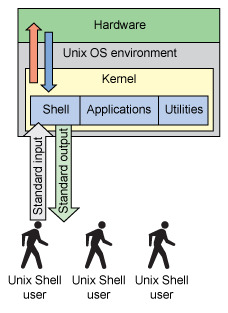
\includegraphics [width=0.6\textwidth , height=0.6\textheight]{figuras/shell_linux.jpg}
%%%prolog/scale=0.47
%\label{fig_solutions_covering}
\caption{Linux x Hardware}
\end{figure}





\section{Acesso via Terminal ou Consoles}

\begin{figure}[!htb]
\centering
%%\includegraphics[width=0.6\textwidth , height=0.5\textheight]{figuras/trens.png}
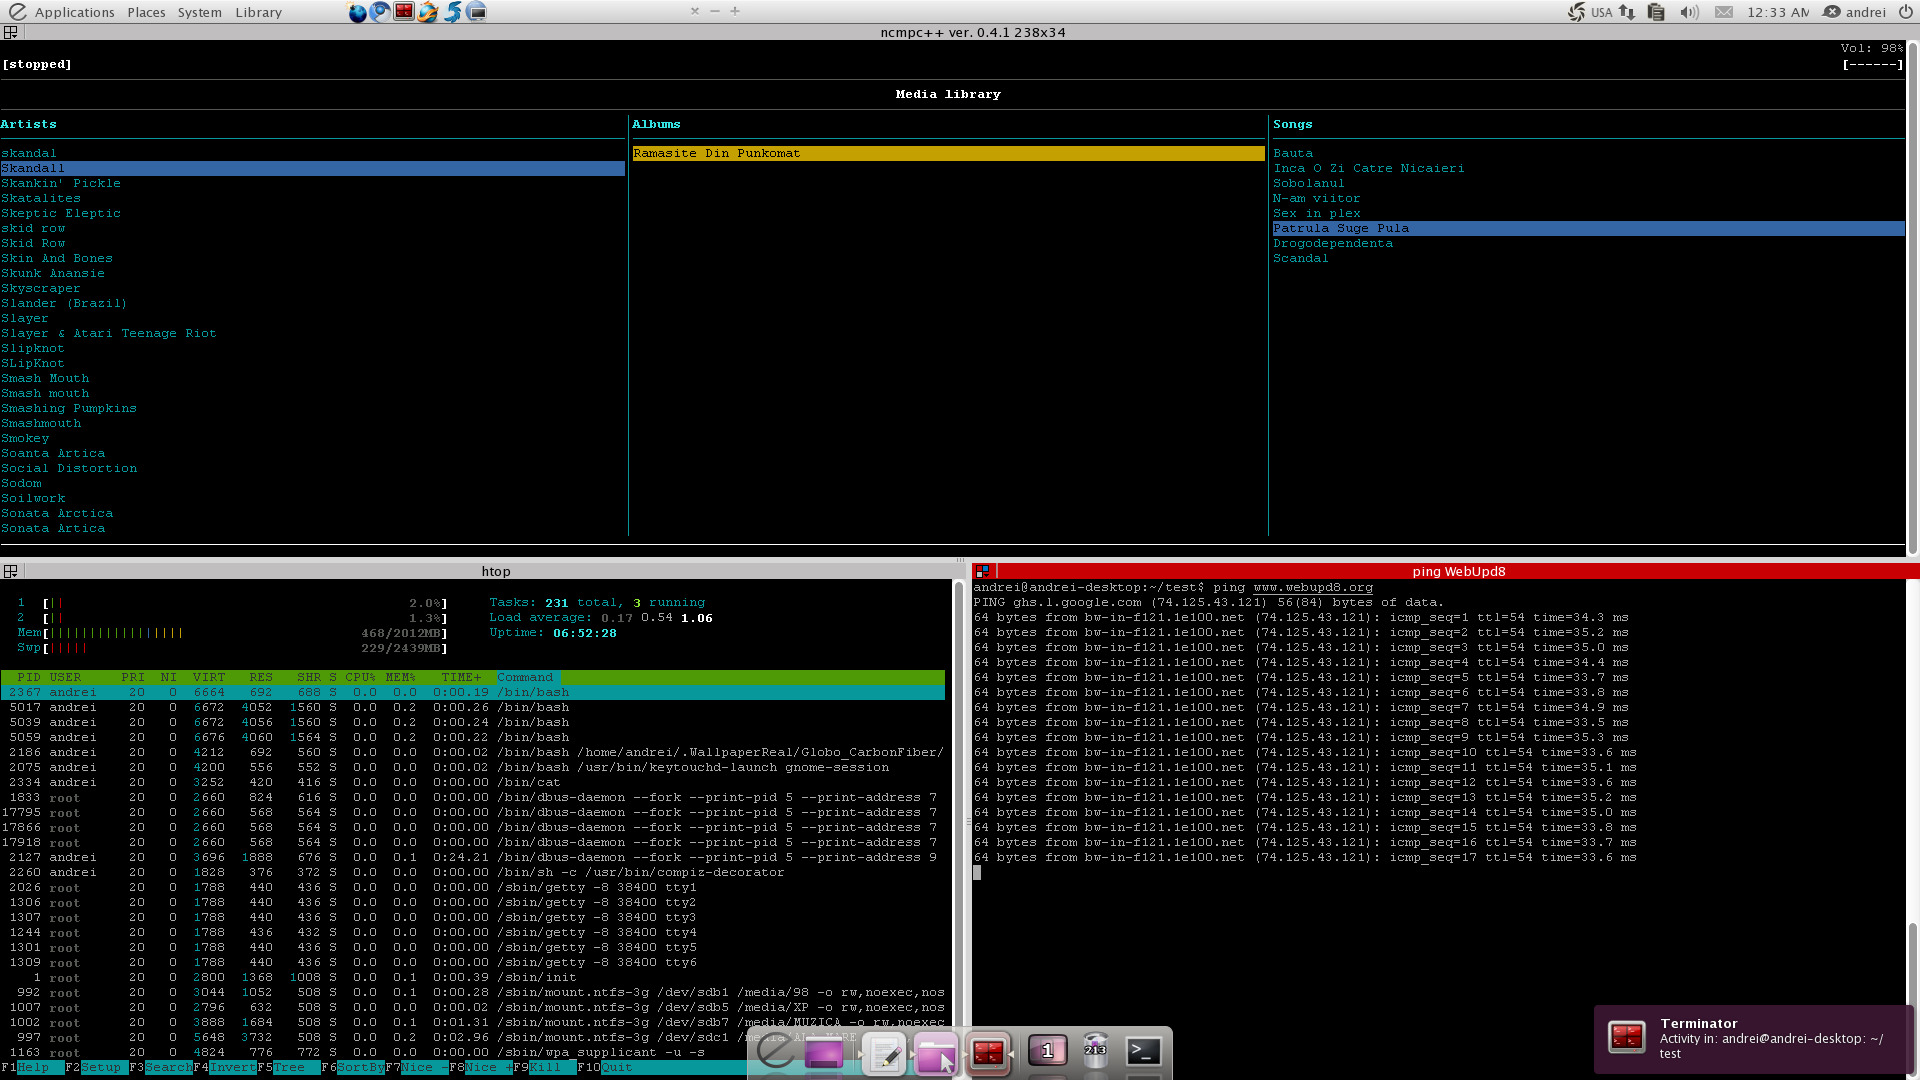
\includegraphics[scale=0.22]{figuras/xterminals.jpg}
%%%prolog/scale=0.47
%\label{fig_solutions_covering}
\caption{Terminal ou Consoles}
\end{figure}



\section{Um Terminal}


\begin{figure}[!htb]
\centering
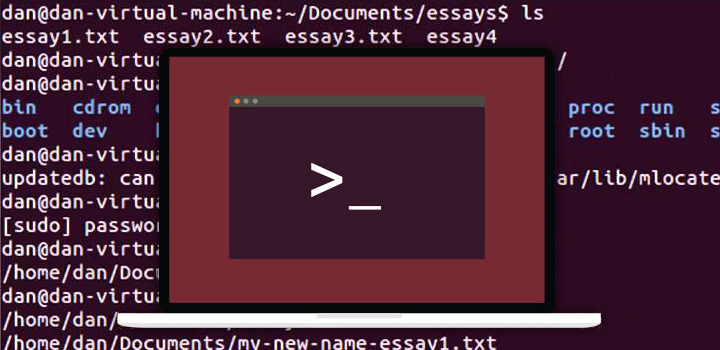
\includegraphics[width=0.6\textwidth , height=0.5\textheight]{figuras/terminal_unico.jpg}
%\includegraphics[scale=0.9]{figuras/trens.pdf}
%%%prolog/scale=0.47
%\label{fig_solutions_covering}
\caption{Isto é uma console ou terminal (\textit{o fim do mundo!})}
\end{figure}


\section{Comandos no Linux}

\begin{enumerate}
  \item Vão ocorrer nesta linha de comando
  \item Voce terá que aprender e decorar uns comandos (traga um \textit{datashet})
  \item Estes comandos serão interpretados pelo programa \textit{bash}, o qual
  acionam o \textit{kernel} linux
  \item e só!
\end{enumerate}



\section{As Teclas}


\begin{itemize}
  \item No linux as teclas também ocupam o lugar do \textit{mouse}, estas
s\~ao \textbf{aceleradoras}

\item \textcolor{red}{Quando tiveres prática, o \textit{rato} fica em segundo momento!}

\end{itemize}

Começando:
\begin{description}


\item[\texttt{xterm} ou \texttt{lxterminal}:] aplicativo terminal (aqui faz tudo!)
\item[Cursor $+$ botão do meio:]  \textit{copy-paste} ao ter um texto marcado
\item[Alt $+$ Tab:] alterna entre as aplicações ativas

\item[$\uparrow $ e $\downarrow $:] repetem os comandos digitados neste terminal
\item[\texttt{\^}: ] é o \texttt{ENTER} o qual deve ser pressionado após os comandos
que se seguem

\end{description}


\section{Estendendo estes atalhos de teclado}

\underline{\textbf{Sobre processos}}:
\begin{description}
\item[\texttt{Ctrl+C}:] Mata um processo sob o aplicativo terminal
\item[\texttt{Ctrl+Z}:] Depois
\item[\texttt{Ctrl+D}:] Fecha a janela terminal (não use), apenas em 
desespero de causa!
\end{description}

\textbf{\textbf{Sobre a tela}}:
\begin{description}
\item[\texttt{Ctrl+L}:] Limpa a tela no terminal (uso bastante)
\item[\texttt{Ctrl+S}:] Faz um \textbf{stop} de uma saída no terminal
\item[\texttt{Ctrl+Q}:] Retoma esta saída pausada na janela terminal \end{description}


\section{Atalhos para mover o cursor}

\underline{\textbf{Atalhos na linha de comando}}:
\begin{description}
\item[\texttt{Ctrl+A} ou \texttt{Home}:] move para o início de linha
\item[\texttt{Ctrl+E} ou \texttt{End}:] move para o fim de linha
\item[\texttt{Ctrl+B}:] move o cursor para palavra \textbf{antes} dele (isto é: à esquerda)
\item[\texttt{Alt+F}:] move o cursor para palavra \textbf{depois} dele
(isto é: à direita)
\item[\texttt{Ctrt+F}:] move o cursor um carácter à \textbf{direita} dele (muito útil)

\item[\texttt{Ctrt+D} ou \texttt{Delete}:] exclui o carácter e puxa-o da direita dele o próximo carácter

\item[\texttt{Alt+D}:] exclui todos carácteres à direita dele

\item[\texttt{Ctrl+H} ou \texttt{Backspace}:] exclui o carácter
antes dele 

\end{description}

\textcolor{red}{Falta ainda o \textit{copy-paste} usando teclas!}



\section{Comandos Introdutórios}

\begin{description}


\item[\ding{248}] Vendo o diretório onde estou:
\begin{verbatim}
$ pwd
/home/udesc
\end{verbatim}


\pagebreak
\item[\ding{248}] Listando o conteúdo do diretório:
\begin{verbatim}
$ ls
......................................................
$ 
TESTE ESTE
$ ls *.txt
......................................................
$ 
TESTE ESTE
$ ls .*
......................................................


\end{verbatim}







\pagebreak
\item[\ding{248}] Cria um diretório
\begin{verbatim}
$ mkdir seu_diretorio
$ ls    
TEM QUE APARECER seu_diretorio LAH
\end{verbatim}


\pagebreak
\item[\ding{248}] Entrando dentro de uma pasta/diretório:
\begin{verbatim}
$ cd seu_diretorio/    VAI para seu diretorio
$ cd ..                SOBE  um nivel acima
$ cd pgms_prolog/      VAI PARA BAIXO ou um dado diretorio
$ cd ~  ATEH RAIZ HOME
$ pwd
/home/udesc
$ 
\end{verbatim}



\pagebreak
\item[\ding{248}] Cria um arquivo e lista o conteúdo:
\begin{verbatim}
$ touch nome_arquivo.txt
$ ls -al *.txt
-rwxr-xr-x 1 udesc udesc 435 2011-08-29 15:34 append.txt
-rw-r--r-- 1 udesc udesc   0 2011-08-29 19:41 nome_arquivo.txt
\end{verbatim}


\pagebreak
\item[\ding{248}] Passos para os laboratórios da turma de ALP (os demais cursos, mais adiante):


\begin{description}

 \setlength\itemsep{13pt}

  \item[\ding{242} \texttt{gterminal}:] é o terminal já mencionado
    \item[\ding{242} \texttt{mkdir SEU\_NOME \^}:] cria diretório
        \item[\ding{242} \texttt{cd SEU\_NOME \^}:] vai para o seu diretório
        \item[\ding{242} \texttt{touch programa.c \^}:] criou um arquivo chamado \texttt{programa.c}
        \item[\ding{242} \texttt{geany programa.c \& \^ }:] edita o \texttt{programa.c} com o \texttt{geany}
       \item[\ding{242} \texttt{gcc programa.c \^ }:] compila o arquivo o \texttt{programa.c} 
    \item[\ding{242}  \texttt{ls a* \^}:] verifica se o programa executável foi gerado, é o \textbf{a.out}  
    \item[\ding{242}  \texttt{./a.out \^}:] executa o \textbf{a.out}  
    \item[\ding{242}  \texttt{ls \* \^}:] lista diretório corrente
       
\end{description}


\pagebreak
\item[\ding{248}] Erro recorrente da turma:



\begin{verbatim}
$ geany nome_arquivo.txt  ^ // processo PARADO
^Z
[1]+  Parado              //geany xxxx   PARADO
$

$ bg 1 ^                    // processo 1 PARADO
[1]+ geany nome_arquivo.txt & ^  // bg ATIVANDO-O

o correto eh:

$ geany nome_arquivo.txt    &  ^   
          
          // NAO ESQUECA O & comercial ao final 
          // ^ eh o ENTER ....

\end{verbatim}


\pagebreak
\item[\ding{248}] Listando processos na memória:
\begin{verbatim}
$ ps 
  PID TTY          TIME CMD
 4685 pts/2    00:00:00 bash
 4790 pts/2    00:00:00 ps

$ ps -aux | grep udesc
........


$ ps -aux | grep udesc | more
.....................
lista os processos por pagina

TESTE
$ htop

\end{verbatim}



\pagebreak
\item[\ding{248}] Processos na memória e seu estado:
\begin{verbatim}

$ ps aux | grep NOME_DO_PROGRAMA
 
SE PARADO, por exemplo: 
$ gedit nome_arquivo.txt   // processo em modo parado
^Z
[1]+  Parado     
$
$ bg 1
[1]+ gedit nome_arquivo.txt &   // posto em background

\end{verbatim}

\pagebreak
\item[\ding{248}] Criar e apagar arquivos  e diretórios:
\begin{verbatim}
$ touch x
$ rm x
$ mkdir cria_diretorio
$ rmdir cria_diretorio
\end{verbatim}

\begin{itemize}
  \item \textcolor{red}{Diretórios só apagam se estiverem vazios!}
   \item \textcolor{red}{\textbf{NUNCA}:} \texttt{rm $\ast$} muito menos \texttt{rm -r $\ast$}
\end{itemize}

\pagebreak
\item[\ding{248}] Copiar um arquivo:
\begin{verbatim}
$ cp origem.txt destino.txt
$ cp casa.pdf /media/arch_linux/pgms_prolog/

\end{verbatim}

\pagebreak
\item[\ding{248}] Copiando recursivamente um diretório:
\begin{verbatim}
$ cp -R haskell/ /media/arch_linux/

\end{verbatim}

\pagebreak
\item[\ding{248}] Renomear um arquivo:
\begin{verbatim}
$ mv casa.pdf /media/arch_linux/pgms_prolog/
$ rename atual novo

\end{verbatim}




\pagebreak
\item[\ding{248}] Limpar tela:
\begin{verbatim}
clear
reset

\end{verbatim}


\pagebreak
\item[\ding{248}] Mostrar o conteúdo de um arquivo texto use o comando
\em{more}:
\begin{verbatim}
$ more append.txt 
more 001_tipos_dados_C.c 
#include <stdio.h>
int main()
	{   // INICIO { ... comentado
	  int ANO	              ;
	  float PI = 3.141519141519141519141519 ;
	  char  sexo = 'M'    ; 
	  char  nome[20] = "Isto eh uma string" ; 
	  bool  luz = true    ;
	  // ISTO EH UMA ATRIBUICAO
	  ANO = 2017            ;	  
// ESCRITA DE VALORES	  
/*
 f : eh file = arquivo
 stdin: standard input = teclado
 stdout: standard output = tela
--More--(44%)


\end{verbatim}
Obs: o comando \em{cat} também funciona para qualquer tipo de arquivo!

\pagebreak
\item[\ding{248}] Pesquisar um arquivo com um dado específico:
\begin{verbatim}
$ grep "Y" *.pl
aula-15-08a.pl:			    p(Y), 
aula-15-08a.pl:			    X \== Y, 
aula-15-08a.pl:			    Z is (X + Y) ,
........................................
udesc@matrizubuntu9:~/pgms_prolog$ 

\end{verbatim}

\pagebreak
\item[\ding{248}] Criar um link simbólico ou atalho (em geral se cria este atalho em \texttt{/usr/bin} ou \texttt{/usr/local/bin}). 

\begin{verbatim}
EXEMPLO:
$ ln -s caminho/minizinc minizinc
PERMISSAO DE EXECUCAO:
$ chmod +x minizinc  (em  /usr/bin)
caminho = onde foi instalado o ORIGINAL
\end{verbatim}

\emph{A soft link, or more common, a symlink, is link a shortcut to the targeted file or directory. So when is removed the original target stays present. This is the opposite of a hard link which is a reference to the target and so, if the hard link is removed, so is the target.}

\pagebreak
\item[\ding{248}] Remover um link simbólico ou atalho (não link físico)

\begin{verbatim}
APENAS para o SIMBOLICO ....
$ ln -s caminho/nota_Minizinc_IDE.txt TESTE.TXT
$ rm TESTE.TXT 
$ ls caminho/*.txt
$ nota_Minizinc_IDE.txt
\end{verbatim}

\pagebreak
\item[\ding{248}] Remover um link simbólico ou atalho (não link físico)
com segurança
\begin{verbatim}
$ unlink  link_simbolico_criado
\end{verbatim}
O original ficou intacto!

\end{description}




\newpage
\subsection{Contato:}
UDESC/CCT/DCC \\
Grupo de Hardware e Software Livre -- Colméia\\

\subsection{Sítio de Referência:}

\textsf{http://www.colmeia.udesc.br/}






\end{document}
